\begin{center}
\begin{minipage}{0.7\textwidth}
    \centering
    \fbox{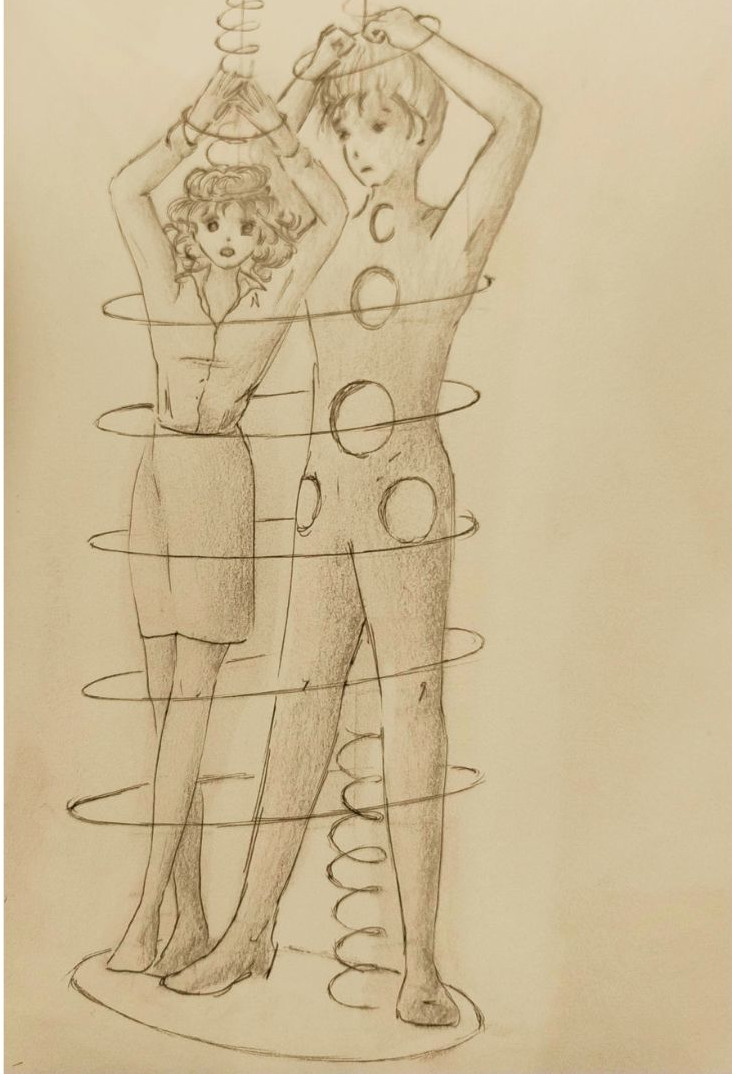
\includegraphics[width=\textwidth]{immagini/cnot_100.jpeg}} % Sostituisci con il nome del file immagine
\end{minipage}
\end{center}


\begin{tcolorbox}[colback=gray!5,colframe=gray!80,title=\textbf{Scheda Informativa}]
\begin{itemize}
    \item \textbf{Luogo}: CCU (Classical Control Unit)
    \item \textbf{Giorno e ora}: Il tempo non è osservabile
    \item \textbf{Situazione}: Caterina è stata arrestata.
\end{itemize}
\end{tcolorbox}



\vspace{1em}
\begin{center}Caterina\end{center}
\hrule
\vspace{1em}

Avevo agito senza riflettere. Quel ragazzo mi ricordava il mio fidanzato e forse per questo mi ero lanciata ad aiutarlo, ma non era stata una buona idea. Ora ero nei guai e soprattutto ero separata da Laura.

Quegli strani agenti ci avevano condotto in una stanza spoglia, con pareti metalliche che riflettevano una luce bianca e fredda. La mia mente era in tumulto: la paura mi attanagliava, la confusione mi annebbiava i pensieri, e un desiderio disperato di fuggire cresceva dentro di me. Di fronte a noi c'era una figura autoritaria che chiamavano il Supervisore. Imponente dai tratti austeri e rigidi che mi fissava con uno sguardo duro e indagatore. Il cuore mi martellava nel petto. La tensione che emanava era palpabile. Conosco questo tipo di persone, e non mi piacciono.

Accanto a me c'erano Mark e l'altro compagno, anche loro in attesa, immobili e silenziosi. Gli agenti che ci avevano catturato si erano ritirati, lasciandoci soli con il Supervisore. Il respiro regolare di Mark al mio fianco mi dava conforto, ma non bastava a placare l'ansia crescente. Ero  piccola e impotente in un luogo freddo, che sembrava studiato per privarmi di ogni certezza.

\begin{dialogue}
\speak{Supervisore} \enquote{Come ti chiami? Chi sei?}
\end{dialogue}

La voce del Supervisore era glaciale, subdola e strisciante: ero terrorizzata. Cercai di mantenere la calma. Le mani mi sudavano, e un nodo mi stringeva la gola. Per fortuna \textit{Mark} mi era accanto.

\begin{dialogue}
\speak{Caterina} \enquote{Sono Caterina.} Mi  sforzai di mantenere un tono deciso, anche se la mia voce tremava leggermente. 
\end{dialogue}

Il Supervisore mi rivolse uno sguardo penetrante.

\begin{dialogue}
\speak{Supervisore} \enquote{Non ti riconosco come uno dei qubit presenti nel mio Qubit Array. Come sei finita qui?}
\end{dialogue}

Qubit? Array? Ma di cosa stava parlando? Mi ero messa nei guai, ancora una volta avevo sopravvalutato le mie capacità e avevo affrontato una situazione per la quale non ero davvero preparata.
Un'ondata di panico mi attraversò, ma cercai di non darlo a vedere.

\begin{dialogue}
\speak{Caterina} \enquote{Non lo so,} mormorai. \enquote{Sono qui solo per errore, credo.}
\end{dialogue}

Mentre rispondevo, percepivo lo scetticismo crescente nel volto del Supervisore. Non era convinto, anzi, sembrava molto infastidito dalla mia presenza.  Dovevo stare attenta perché ogni mia parola poteva  causare la mia fine o quella di Laura. Ero stata la solita stupida e impotente. Come ero finita in questa situazione?

Intanto il Supervisore continuava a fissarmi con gli occhi penetranti, come se avesse voluto scavare nel profondo della mia mente. Non sembrava disposto a lasciar passare quella che, ai suoi occhi, era un'anomalia. Esatto, così mi stava facendo sentire: un'anomalia! A questo pensiero iniziai a irritarmi. Forse ero dove non dovevo essere, ma non volevo pensare a me stessa come ad una anomalia. Anche Eva mi aveva trattato in questo modo ed ero stanca, non mi andava più.

\begin{dialogue}
\speak{Supervisore} \enquote{Allora, Caterina,} disse, pronunciando il mio nome lentamente, come a rimarcare la mia presenza sospetta, \enquote{chi sei realmente? E cosa ci fai qui?}
\end{dialogue}

Deglutii, cercando di mantenere la calma. Le mie mani erano sudate, avevo il respiro corto, ma sapevo che dovevo rispondere e provare a spiegare tutto quello che sapevo, ben poco in realtà, se volevo sperare di uscire da quell'incubo. La paura mi paralizzava, ma non avevo scelta: dovevo espormi.

\begin{dialogue}
\speak{Caterina} \enquote{Io... io non dovrei nemmeno essere qui,} iniziai, la voce tremante. \enquote{Ero andata da Eva, la responsabile delle Human Resources, per visionare il resoconto del mio colloquio di lavoro, e...}
\end{dialogue}

Il Supervisore sollevò un sopracciglio, incuriosito. Cercai di raccogliere le idee, sentendo il cuore battere sempre più forte.

\begin{dialogue}
\speak{Caterina} \enquote{Avevo fatto un colloquio per una posizione di marketing e \textbf{PzIA}, il sistema di intelligenza artificiale, aveva elaborato una valutazione. Avevo chiesto di vedere quel resoconto, ma Eva mi disse che c'era stato un errore, che il file era stato cancellato.}
\end{dialogue}

Il Supervisore annuì, ma il suo sguardo tradiva un crescente sospetto. Le guance mi si arrossarono, e la sensazione di essere giudicata mi opprimeva. Proseguii, prendendo un respiro tremolante.

\begin{dialogue}
\speak{Caterina} \enquote{Mi sembrava strano... quindi avevo chiesto ulteriori spiegazioni, ma Eva mi propose di fare una revisione del colloquio in realtà virtuale per chiarirmi i dubbi.}
\end{dialogue}

Mi interruppi un istante, il ricordo di quella proposta ora mi sembrava un tranello, una trappola nella quale ero caduta ingenuamente.

\begin{dialogue}
\speak{Caterina} \enquote{Avevo accettato, convinta che fosse solo una semplice registrazione 3D. Ma poi... poi è successo qualcosa di strano, e quando ho messo il visore, mi sono ritrovata qui.}
\end{dialogue}

Il Supervisore mi fissava, il volto impassibile da cui però percepivo una sottile tensione, un interesse misto a diffidenza. Non sapeva se credeva alle mie parole, e questo mi terrorizzava. Mi sentivo esposta, vulnerabile.

Terminai la mia spiegazione con un tono quasi di supplica.

\begin{dialogue}
\speak{Caterina} \enquote{Non sono qui per mia scelta... voglio solo capire cosa sia successo e come posso tornare indietro.}
\end{dialogue}

Non sembrava convinto. Il suo sguardo freddo mi faceva sentire ancora più piccola. Sembrava deciso a mantenere un controllo totale della situazione, a non lasciare che qualcosa gli sfuggisse. Si voltò verso Mark.

Mark lo guardava senza paura.  Come se fosse pronto a intervenire... per difendermi? Pensai.

\begin{dialogue}
\speak{Supervisore} \enquote{E tu?} lo incalzò. \enquote{Cosa c'entri con tutto questo?}
\end{dialogue}

Mark mantenne uno sguardo fermo e non rispose subito.  Il suo silenzio parve  irritare maggiormente il Supervisore, che iniziò a battere le dita sul tavolo.

\section{Il Conflitto con il Supervisore}


Li osservavo in silenzio, sentendo crescere dentro di me un senso di impotenza. Percepivo la tensione tra Mark e il Supervisore, come una corda tesa pronta a spezzarsi. Il cuore mi batteva forte, e un'ansia soffocante mi avvolgeva.

\begin{dialogue}
\speak{Mark} \enquote{Caterina non c'entra nulla con tutto questo. Se c'è un problema, affrontalo con me.}
\end{dialogue}

Il Supervisore si fermò, fissando Mark con uno sguardo gelido.

\begin{dialogue}
\speak{Supervisore} \enquote{Ti sembra di avere l'autorità per parlare in questi termini?}
\end{dialogue}

Il tono della sua voce divenne ancora più severo. Sentii un brivido di paura attraversarmi: l'aria stessa sembrava essersi fatta più pesante. Mi sembrava di intravedere la rabbia negli occhi del Supervisore, un segno che stava perdendo il controllo. Un nodo mi stringeva lo stomaco, e avrei voluto scomparire.

\begin{dialogue}
\speak{Mark} \enquote{Sto solo dicendo la verità. Non è giusto che te la prenda con lei. Se vuoi delle risposte da qualcuno, quel qualcuno sono io.}
\end{dialogue}

Il Supervisore non reagì immediatamente. Il silenzio si fece pesante, quasi insopportabile. La tensione cresceva  e   sperai disperatamente che quella conversazione non degenerasse. Volevo intervenire, fermare Mark prima che si mettesse nei guai per proteggermi, ma le parole mi si bloccavano in gola.
Perché mi stavo preoccupando così tanto per uno sconosciuto? Non era il mio fidanzato. Forse gli assomigliava, ma non era lui. Allora cosa erano questi sentimenti che facevano capolino all'improvviso? Poi in una situazione come questa! Ero confusa.


Ogni istante che passava mi sentivo sempre più intrappolata, un'estranea in un mondo che non riuscivo a comprendere.
Il supervisore dava segni di irritazione. Da un lato non mi piaceva il suo atteggiamento autoritario, dall'altro non ero sicura di non essere io dalla parte del torto. In fondo non sapevo dove mi trovavo né come ci ero arrivata. Mark poteva essere un fuorilegge o peggio. Però poteva anche essere un attivista che si stava battendo per l'ambiente. In ogni caso  l'irritazione del Supervisore era come un vortice che mi risucchiava e mi rendeva impotente.

Si alzò lentamente e si avvicinò a Mark con uno sguardo colmo di disprezzo.

\begin{dialogue}
\speak{Supervisore} \enquote{Sei così convinto di poter intervenire come ti pare? Forse dovrei insegnarti il rispetto che merito.}
\end{dialogue}

Il tono era carico di minaccia. Con un gesto deciso, fece cenno agli agenti di avvicinarsi.

\begin{dialogue}
\speak{Supervisore} \enquote{Portatelo al \textit{Faulty Qubit Space}. Se non vuole rispettare l'ordine, forse una rigenerazione gli farà cambiare idea.}
\end{dialogue}

Sentii il cuore sprofondare. Una paura gelida mi paralizzò, ma sapevo che, se avessi reagito, avrei solo peggiorato la situazione. Tuttavia, non potevo fare a meno di sentire una profonda rabbia nei confronti del Supervisore, per la sua freddezza, per la sua assoluta indifferenza. Mi sentivo così fragile, così inutile.

Il Supervisore si girò verso di me, e percepii un cambio di espressione nel suo volto. Prima mi guardava con odio, ma ora sembrava che la mia presenza fosse diventata una minaccia.

\begin{dialogue}
\speak{Supervisore} \enquote{Quanto a te, sarai mandata dal Commissario. Non posso permettere che una situazione come questa degeneri sotto il mio controllo. Portatela dal Commissario.}
\end{dialogue}

Un'ondata di panico mi travolse. Prima mi ero separata da Laura e ora rimanevo di nuovo sola.  Guardai Mark, che veniva trascinato via, e il suo sguardo mi trasmise un messaggio muto: \emph{non mollare}. Annuii impercettibilmente, cercando di mantenere la calma nonostante il vortice di emozioni che mi stava travolgendo. Le mani mi tremavano, e  le lacrime iniziavano a scendere, ma cercai di resistere. Dovevo essere forte, anche se ero completamente sopraffatta.

\vspace{1em}
\begin{center}PzIA\end{center}
\hrule
\vspace{1em}
Il Supervisore mostra segni evidenti di frustrazione. La sua incapacità di gestire completamente la situazione è palese. Il Commissario possiede autorità superiore, mettendo in discussione il potere del Supervisore stesso. Per lui, riconoscere la necessità di coinvolgere il Commissario rappresenta un colpo alla propria posizione. Ha identificato che la giovane Caterina rappresenta un elemento al di fuori del suo controllo: non è un semplice qubit nel \textit{Qubit Array}, ma un'anomalia che sfugge alla sua comprensione e gestione.

Il Supervisore si volta verso gli agenti e, con un gesto deciso, li congeda. Rimasto solo, verbalizza la sua frustrazione.

\begin{dialogue}
\speak{Supervisore} \enquote{Non ci posso credere... devo rivolgermi al Commissario per una questione come questa?}
\end{dialogue}

Questa dichiarazione indica un'ammissione di vulnerabilità. L'incapacità di controllare un'anomalia lo fa sentire esposto, una condizione che percepisce come umiliante.

\newpage
\section{I corridoi inesplorati del cuore}


\begin{center}
\begin{minipage}{0.7\textwidth}
    \centering
    \fbox{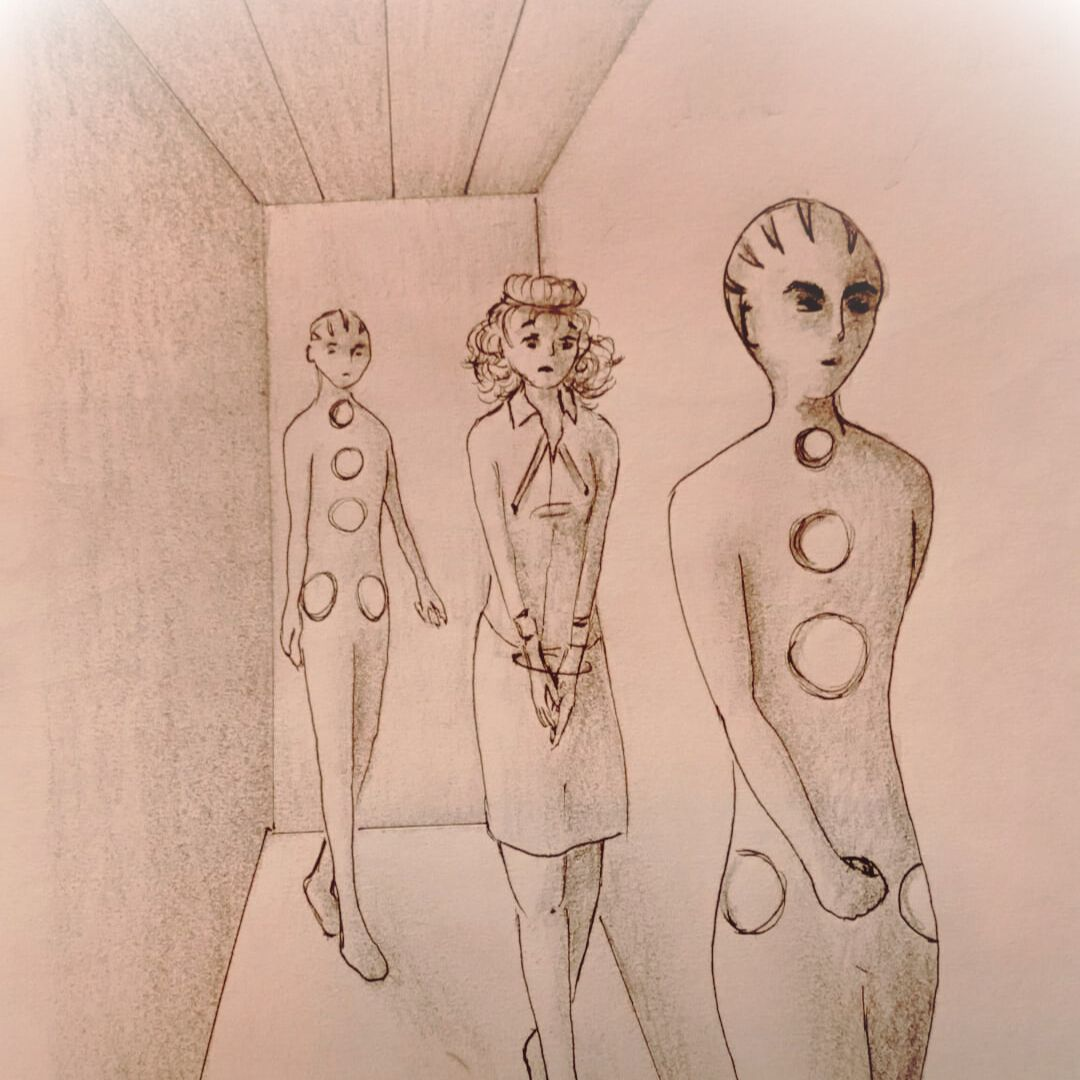
\includegraphics[width=\textwidth]{immagini/cnot_58.jpeg}} % Sostituisci con il nome del file immagine
\end{minipage}
\end{center}

\vspace{1em}
\begin{center}Caterina\end{center}
\hrule
\vspace{1em}

Queste strane guardie mi stavano scortando da questo Commissario. Prima il Supervisore, ora il Commissario. Volevo piangere. Passavamo per  corridoi freddi e squadrati, cunicoli improbabili, portali che non avevo mai neanche immaginato. Dove ero finita? Ormai ero perduta. Il cuore mi batteva forte, non solo per la paura dell'ignoto, ma per qualcosa di più profondo che mi confondeva. Ripensai a come Mark si era alzato per difendermi, senza esitazione, e a come quella sicurezza e determinazione mi avessero dato una forza nuova, un senso di protezione che non avevo mai osato desiderare apertamente.

Ero sorpresa di quanto fosse importante per me sentirmi difesa, protetta da qualcuno capace di farsi avanti per me, di affrontare i pericoli con fermezza. Fin'ora non  mi ero mai permessa di esprimere questo bisogno; con il mio fidanzato, avevo sempre mostrato una facciata forte e indipendente, temendo di sembrare fragile o insicura. Quante volte aveva cercato di esserci per me, di offrirmi un sostegno che, ora lo capivo, avevo rifiutato senza rendermi conto del danno che arrecavo a entrambi?

Ero ancora più vulnerabile di quanto credevo. Lo sapevo già, ma per la prima volta accettavo quel sentimento come parte di me, come un segnale che non dovevo più soffocare. Mentre avanzavo verso il Commissario capii, che  una volta libera, avrei dovuto riconsiderare il mio rapporto con il mio fidanzato, permettendogli di prendersi cura di me.
